\documentclass{libs/XJTLU_format}

%\documentclass{article}

%%%%%%%%%%%%%%%%%%%%%%%%%%%%%%%%%%%%%%%%%%%%%%%%%%%%%%%%%%%%%%%%%%%%%%%%%%%%%%
% \embedvideo{<poster or text>}{<video file (MP4+H264)>}
%%%%%%%%%%%%%%%%%%%%%%%%%%%%%%%%%%%%%%%%%%%%%%%%%%%%%%%%%%%%%%%%%%%%%%%%%%%%%%
\usepackage[bigfiles]{pdfbase}
\usepackage{amssymb}
\ExplSyntaxOn
%%begin novalidate
\cs_new:Npn\embedvideo#1#2{
%%end novalidate
  \leavevmode
  \pbs_pdfobj:nnn{}{fstream}{{}{#2}}
  \pbs_pdfobj:nnn{}{dict}{
    /Type/Filespec/F~(#2)/UF~(#2)
    /EF~<</F~\pbs_pdflastobj:>>
  }
  \tl_set:Nx\video{\pbs_pdflastobj:}%
  %
  \pbs_pdfobj:nnn{}{dict}{
    /Type/RichMediaInstance/Subtype/Video
    /Asset~\video
    /Params~<</Binding/Foreground>>
  }
  %
  \pbs_pdfobj:nnn{}{dict}{
    /Type/RichMediaConfiguration/Subtype/Video
    /Instances~[\pbs_pdflastobj:]
  }
  %
  \pbs_pdfobj:nnn{}{dict}{
    /Type/RichMediaContent
    /Assets~<<
      /Names~[(#2)~\video]
    >>
    /Configurations~[\pbs_pdflastobj:]
  }
  \tl_set:Nx\rmcontent{\pbs_pdflastobj:}%
  %
  \pbs_pdfobj:nnn{}{dict}{
    /Activation~<<
      /Condition/XA
      /Presentation~<<
        /Transparent~true
        /Style/Embedded
        /PassContextClick~true
      >>
    >>
    /Deactivation~<</Condition/PC>>
  }
  %
  \hbox_set:Nn\l_tmpa_box{#1}
  \tl_set:Nx\l_box_wd_tl{\dim_use:N\box_wd:N\l_tmpa_box}
  \tl_set:Nx\l_box_ht_tl{\dim_use:N\box_ht:N\l_tmpa_box}
  \tl_set:Nx\l_box_dp_tl{\dim_use:N\box_dp:N\l_tmpa_box}
  \pbs_pdfxform:nnnnn{1}{1}{}{}{\l_tmpa_box}
  %
  \pbs_pdfannot:nnnn{\l_box_wd_tl}{\l_box_ht_tl}{\l_box_dp_tl}{
    /Subtype/RichMedia
    /BS~<</W~0/S/S>>
    /Contents~(embedded~video~file:#2)
    /NM~(rma:#2)
    /AP~<</N~\pbs_pdflastxform:>>
    /RichMediaSettings~\pbs_pdflastobj:
    /RichMediaContent~\rmcontent
  }
  \phantom{#1}
}%
\ExplSyntaxOff
%%%%%%%%%%%%%%%%%%%%%%%%%%%%%%%%%%%%%%%%%%%%%%%%%%%%%%%%%%%%%%%%%%%%%%%%%%%%%%


% % Inserting the preamble file with the packages
% %%%%%%%%%%%%%%%%%%%%%%%%%%%%%%%%%%%%%%%%%%%%%%%%%%%%%%%%%%%%%%%%%%%%%
%% This file contains the packages that can be used in the beamer. %%
%%%%%%%%%%%%%%%%%%%%%%%%%%%%%%%%%%%%%%%%%%%%%%%%%%%%%%%%%%%%%%%%%%%%%
% Package to fonts family
\usepackage[T1]{fontenc}
% Package to accentuation
\usepackage[utf8]{inputenc}
% Package to Figures
\usepackage{graphicx}
% Package to the colors
\usepackage{color}
% Package to the colors
\usepackage{xcolor}
% Packages to math symbols and expressions
\usepackage{amsfonts, amssymb, amsmath}
% Package to multiple lines and columns in table
\usepackage{multirow, array} 
% Package to create pseudo-code
% For more detail of this package: http://linorg.usp.br/CTAN/macros/latex/contrib/algorithm2e/doc/algorithm2e.pdf
\usepackage{algorithm2e}
% Package to insert code
\usepackage{listings} 
\usepackage{keyval}
% Package to justify text
\usepackage[document]{ragged2e}
% Package to manage the bibliography
\usepackage[backend=biber, style=numeric, sorting=none]{biblatex}
% Package to facilities quotations
\usepackage{csquotes}
% Package to use multicols
\usepackage{multicol}
\usepackage{transparent}

% % Inserting the references file
% \bibliography{references.bib}

% % Title
% \title[MAT 214_Processing and Properties of Ceramic Materials]{\textbf{MAT 214: Processing and Properties of Ceramic Materials}}
% % Subtitle
% \subtitle{Introduction to Ceramic Materials}
% % Author of the presentation
% \author{Prof. Joshua C. Agar}
% % Institute's Name
% \institute[Lehigh University]{
%     % email for contact
%     \normalsize{\email{jca318@lehigh.edu}}
%     \newline
%     % Department Name
%     \department{Materials Science and Engineering}
%     \newline
%     % University name
%     \university{Lehigh Univeristy}
% }
% % date of the presentation
% \date{\today}

% %\newcommand*{\keys}{\fontfamily{cmtt}\selectfont}

%%%%%%%%%%%%%%%%%%%%%%%%%%%%%%%%%%%%%%%%%%%%%%%%%%%%%%%%%%%%%%%%%%%%%%%%%%%%%%


% Inserting the preamble file with the packages
%%%%%%%%%%%%%%%%%%%%%%%%%%%%%%%%%%%%%%%%%%%%%%%%%%%%%%%%%%%%%%%%%%%%%
%% This file contains the packages that can be used in the beamer. %%
%%%%%%%%%%%%%%%%%%%%%%%%%%%%%%%%%%%%%%%%%%%%%%%%%%%%%%%%%%%%%%%%%%%%%
% Package to fonts family
\usepackage[T1]{fontenc}
% Package to accentuation
\usepackage[utf8]{inputenc}
% Package to Figures
\usepackage{graphicx}
% Package to the colors
\usepackage{color}
% Package to the colors
\usepackage{xcolor}
% Packages to math symbols and expressions
\usepackage{amsfonts, amssymb, amsmath}
% Package to multiple lines and columns in table
\usepackage{multirow, array} 
% Package to create pseudo-code
% For more detail of this package: http://linorg.usp.br/CTAN/macros/latex/contrib/algorithm2e/doc/algorithm2e.pdf
\usepackage{algorithm2e}
% Package to insert code
\usepackage{listings} 
\usepackage{keyval}
% Package to justify text
\usepackage[document]{ragged2e}
% Package to manage the bibliography
\usepackage[backend=biber, style=numeric, sorting=none]{biblatex}
% Package to facilities quotations
\usepackage{csquotes}
% Package to use multicols
\usepackage{multicol}
\usepackage{transparent}

% Inserting the references file
\bibliography{references.bib}

% Title
\title[MAT 214 Spring 2022]{\textbf{MAT 214: Processing and Properties of Ceramic Materials}}
% Subtitle
\subtitle{Introduction to Ceramic Materials}
% Author of the presentation
\author{Prof. Joshua C. Agar}
% Institute's Name
\institute[Lehigh University]{
    % email for contact
    \normalsize{\email{jca318@lehigh.edu}}
    \newline
    % Department Name
    \department{Materials Science and Engineering}
    \newline
    % University name
    \university{Lehigh University}
}
% date of the presentation
\date{\today}

%%%%%%%%%%%%%%%%%%%%%%%%%%%%%%%%%%%%%%%%%%%%%%%%%%%%%%%%%%%%%%%%%%%%%%%%%%%%%%%%%%
%% Start Document of the Presentation                                           %%               
%%%%%%%%%%%%%%%%%%%%%%%%%%%%%%%%%%%%%%%%%%%%%%%%%%%%%%%%%%%%%%%%%%%%%%%%%%%%%%%%%%
\begin{document}

% insert the code style
%%%%%%%%%%%%%%%%%%%%%%%%%%%%%%%%%%%%%%%%%%%%%%%%%%%%%%%%%%%%%%%%%%%%%%%%%%%%%%%%%%%
%% This file contains the style of the codes show in slides.                     %%
%% The package used is listings, but it possible to used others.                 %%
%%%%%%%%%%%%%%%%%%%%%%%%%%%%%%%%%%%%%%%%%%%%%%%%%%%%%%%%%%%%%%%%%%%%%%%%%%%%%%%%%%%

% color used in the code style
\definecolor{codegreen}{rgb}{0,0.6,0}
\definecolor{codegray}{rgb}{0.5,0.5,0.5}
\definecolor{codepurple}{rgb}{0.58,0,0.82}
\definecolor{codebackground}{rgb}{0.95,0.95,0.92}

% style of the code!
\lstdefinestyle{codestyle}{
    backgroundcolor=\color{codebackground},   
    commentstyle=\color{codegreen},
    keywordstyle=\color{magenta},
    numberstyle=\tiny\color{codegray},
    stringstyle=\color{codepurple},
    basicstyle=\ttfamily\footnotesize,
    frame=single,
    breakatwhitespace=false,         
    breaklines=true,                 
    captionpos=b,                    
    keepspaces=true,                 
    numbers=left,                    
    numbersep=5pt,                  
    showspaces=false,                
    showstringspaces=false,
    showtabs=false,                  
    tabsize=2,
    title=\lstname 
}

\lstset{style=codestyle}


%% ---------------------------------------------------------------------------
% First frame (with tile, subtitle, ...)
\begin{frame}{}
    \maketitle
\end{frame}

\section{Learning Objectives}
\begin{frame}{Learning Objectives}
    \begin{itemize}
    \item Understand the difference classes of materials. What makes a ceramic a ceramic?  \pause
    \item Understanding of the diverse types of properties that ceramics can exhibit  \pause
    \item Appreciation for applications and growth opportunities for ceramic materials and industries
\end{itemize}
\end{frame}


\section{Materials Classes}

\begin{frame}{Classes of Materials}
What are the classes of materials? 
\pause

\begin{enumerate}
    \item Metals \pause
    \item Polymer \pause
    \item Ceramics \pause
    \item Semiconductor \pause
    \item Composites \pause
    \item Biomaterials???? \pause
\end{enumerate}

\pause
What is unique about the first three? 

\pause
\hspace{1em}\emph{These are all defined by the nature of the atomic bonding}\\[0.1cm]

\pause
Semiconductors, composites, and biomaterials are defined by their properties

\end{frame}

\begin{frame}{Metals}

\centering
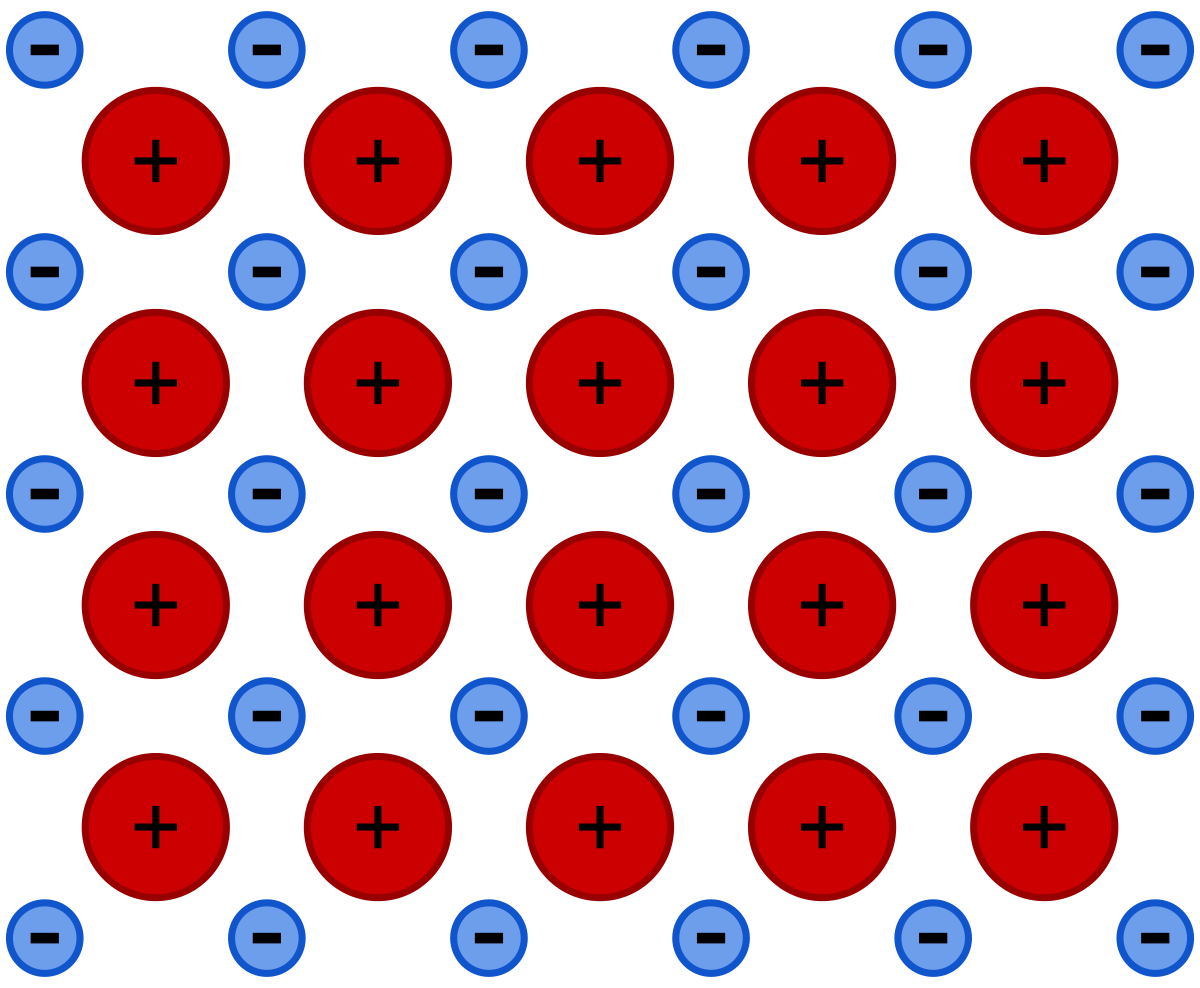
\includegraphics[height=1in]{Silde_Template/images/Metallic_Bonding_Example.svg.png}

\begin{itemize}
    \item Constructed of atoms held together by delocalized electrons
    \pause
    \item They are commonly found as alloys with metallic and non-metallic elements
    \pause
    \item Delocalized electrons give metallic properties (e.g., good thermal and electrical conductivity)
    \pause
    \item Metallic bonding allows for closed-packed crystal structures that permit plastic deformation
\end{itemize}
    
\end{frame}

\begin{frame}{Polymers}

\centering
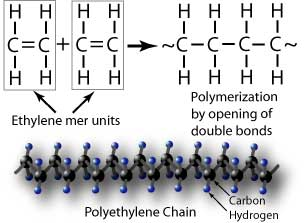
\includegraphics[height=1in]{Silde_Template/images/PolyethyleneChain.jpg}

\begin{itemize}
    \item Macromolecules formed by covalent bonding of many simpler molecular units called mers 
    \pause
    \item Most polymers are organic compounds based on carbon, hydrogen, and other nonmetals such as sulfur and chlorine 
    \pause
    \item The bonding between the molecular chains determines many of their properties
    \pause
    \item Many of the plastics that we are familiar with are actually combinations of polymers and often include fillers and other additives to give the desired properties and appearance
\end{itemize}
\end{frame}

\begin{frame}{Ceramics}
What are ceramics? 
\pause
\vspace{1em}

\begin{itemize}
    \item “Mixed” bonding a combination of covalent, ionic, and sometimes metallic
    \pause
    \item They consist of arrays of interconnected atoms; there are no discrete molecules
    \item The majority of ceramics are compounds of metals or metalloids and nonmetals
    \pause
    \item Most frequently they are oxides, nitrides, and carbides, however, diamond and graphite are considered ceramics.
\end{itemize}
\pause

\vspace{1em}
\textbf{Most solid materials that are not metal, plastic, or derived from plants or animals are ceramics}

\end{frame}

\begin{frame}{Semiconductors}

\centering
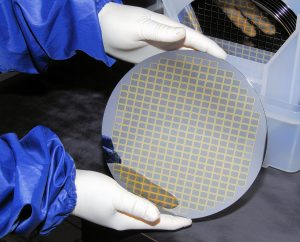
\includegraphics[height=1in]{Silde_Template/images/Wafer.jpg}

\begin{itemize}
    \item Only class of material based on a property
    \pause
    \item They are usually defined as having electrical conductivity between that of a good conductor and an insulator
    \pause
    \item The conductivity is strongly dependent upon the presence of small amounts of impurities
    \pause
    \item Classically, semiconductors have been limited to materials with a band gap $<3eV$, but there is growing commercial interest in large band gap semiconductors for high-temperature electronics.
\end{itemize}
    
\end{frame}

\begin{frame}{Composites}
    \centering
    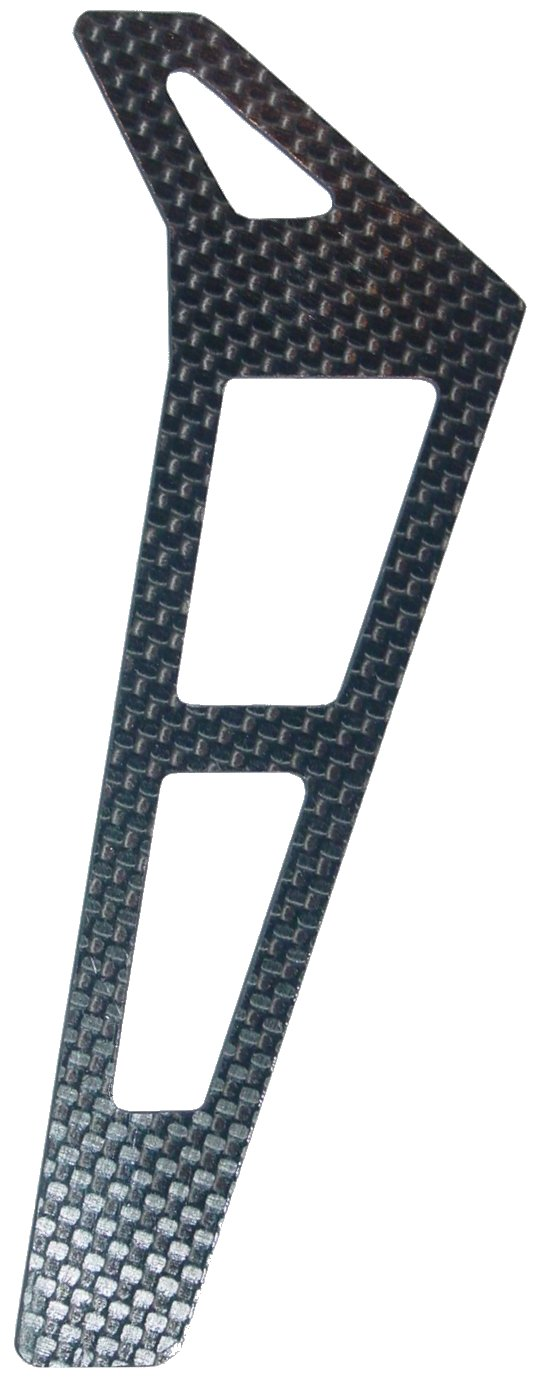
\includegraphics[height=1in]{Silde_Template/images/carbon_fiber.jpeg}

    \begin{itemize}
        \item Composites are materials formed by more than one material (sometimes this is extended to phase)
        \pause
        \item Usually there is a matrix and a filler
        \pause
        \item It is quite common to have ceramic composites
    \end{itemize}
    
    
\end{frame}

\begin{frame}{Ceramic Ontologies and Exceptions}
Exclusionary definition: Ceramic materials are inorganic, non-metallic solids.
\pause

\begin{itemize}
    \item All inorganic semiconductors are ceramics
    \pause
    \item A materials ceases to be a ceramic when melted
    \pause
    \item All high-temperature superconductors are ceramics
    \pause
    \item Ice even though it is an inorganic material in the solid phase is not a ceramic
    \pause
    \item Glasses live in a gray area - it is really a supercooled liquid
\end{itemize}
    
\end{frame}

\begin{frame}{Ceramic Ontologies and Exceptions}
Ceramics cannot be defined based on their properties

\begin{itemize}
    \item We can’t say “ceramics are brittle” because some can be superplastically deformed and some metals can be more brittle: a rubber hose or banana at 77 K shatters under a hammer
    \pause
    \item We can’t say “ceramics are insulators” unless we put a value on the band gap (Eg) where a material is not a semiconductor.
    \pause
    \item We can’t say “ceramics are poor conductors of heat” because diamond has the highest thermal conductivity of any known material. Porous ceramics have some of the lowest thermal conductivity of any known materials.
\end{itemize}
    
\end{frame}

\section{Properties of Ceramics}

\begin{frame}{Brittleness}
    \centering
    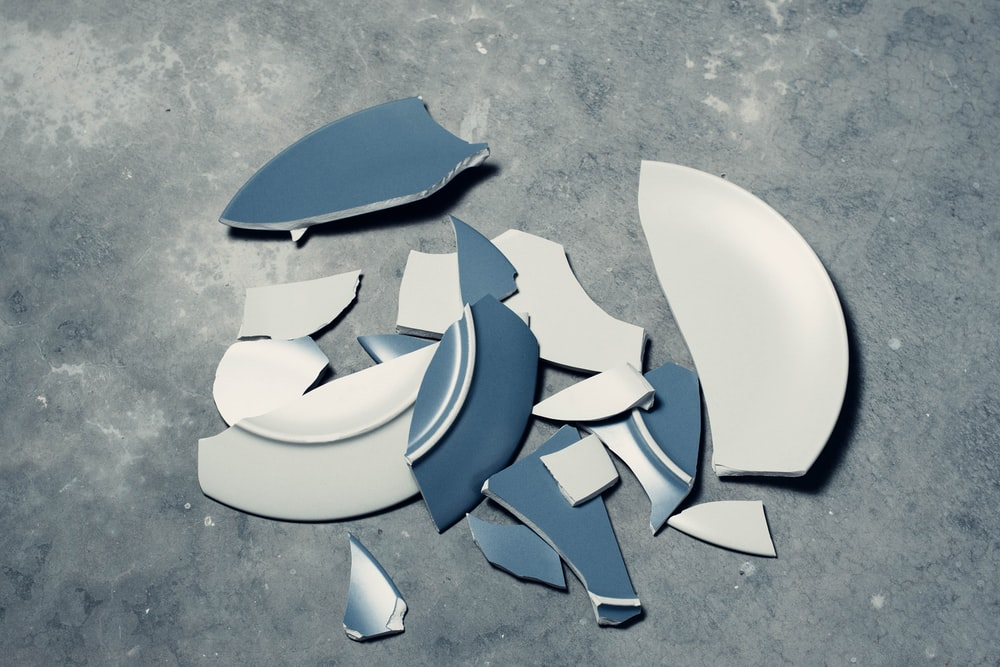
\includegraphics[height=1in]{Silde_Template/images/plate.jpeg}
    
    \begin{itemize}
        \item This property is recognized from personal experience, such as dropping a glass beaker or a dinner plate
        \pause
        \item The reason that the majority of ceramics are brittle is the mixed ionic-covalent bonding that holds the constituent atoms together
        \pause
        \item Most ceramics are brittle at room temperature but not necessarily at elevated temperatures -- they can become viscous
    \end{itemize}
    
\end{frame}

\begin{frame}{Poor Electrical and Thermal Conduction}
    
    \begin{itemize}
        \item The valence electrons are tied up in bonds and are not free as they are in metals
        \pause
        \item Diamond, which we classified as a ceramic, has the highest thermal conductivity of any known material. \pause The conduction mechanism is due to phonons, not electrons.
        \pause
        \item The oxide ceramic $ReO_{3}$ has an electrical conductivity at room temperature similar to that of Cu
        \pause
        \item The mixed oxide $YBa_{2}Cu_{3}O_{7}$ is an HTSC; it has zero resistivity below 92 K
    \end{itemize}
    
\end{frame}

\begin{frame}{Compressive Strength}
    \centering
    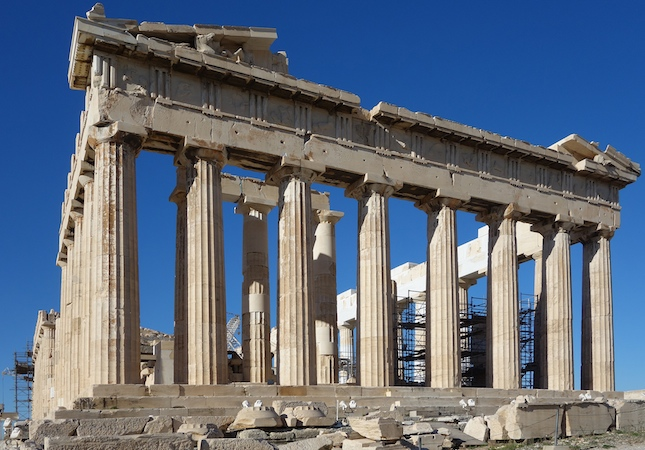
\includegraphics[height=1in]{Silde_Template/images/Greekcolumns.jpeg}
    
    \begin{itemize}
        \item Ceramics are stronger in compression than in tension, whereas metals have comparable tensile and compressive strengths \pause
        \item This difference is important when we use ceramic components for load-bearing applications \pause
        \item Ceramics generally have a low degree of toughness, although combining them in composites can dramatically improve this property
    \end{itemize}
\end{frame}

\begin{frame}{Chemical insensitivity}

\centering
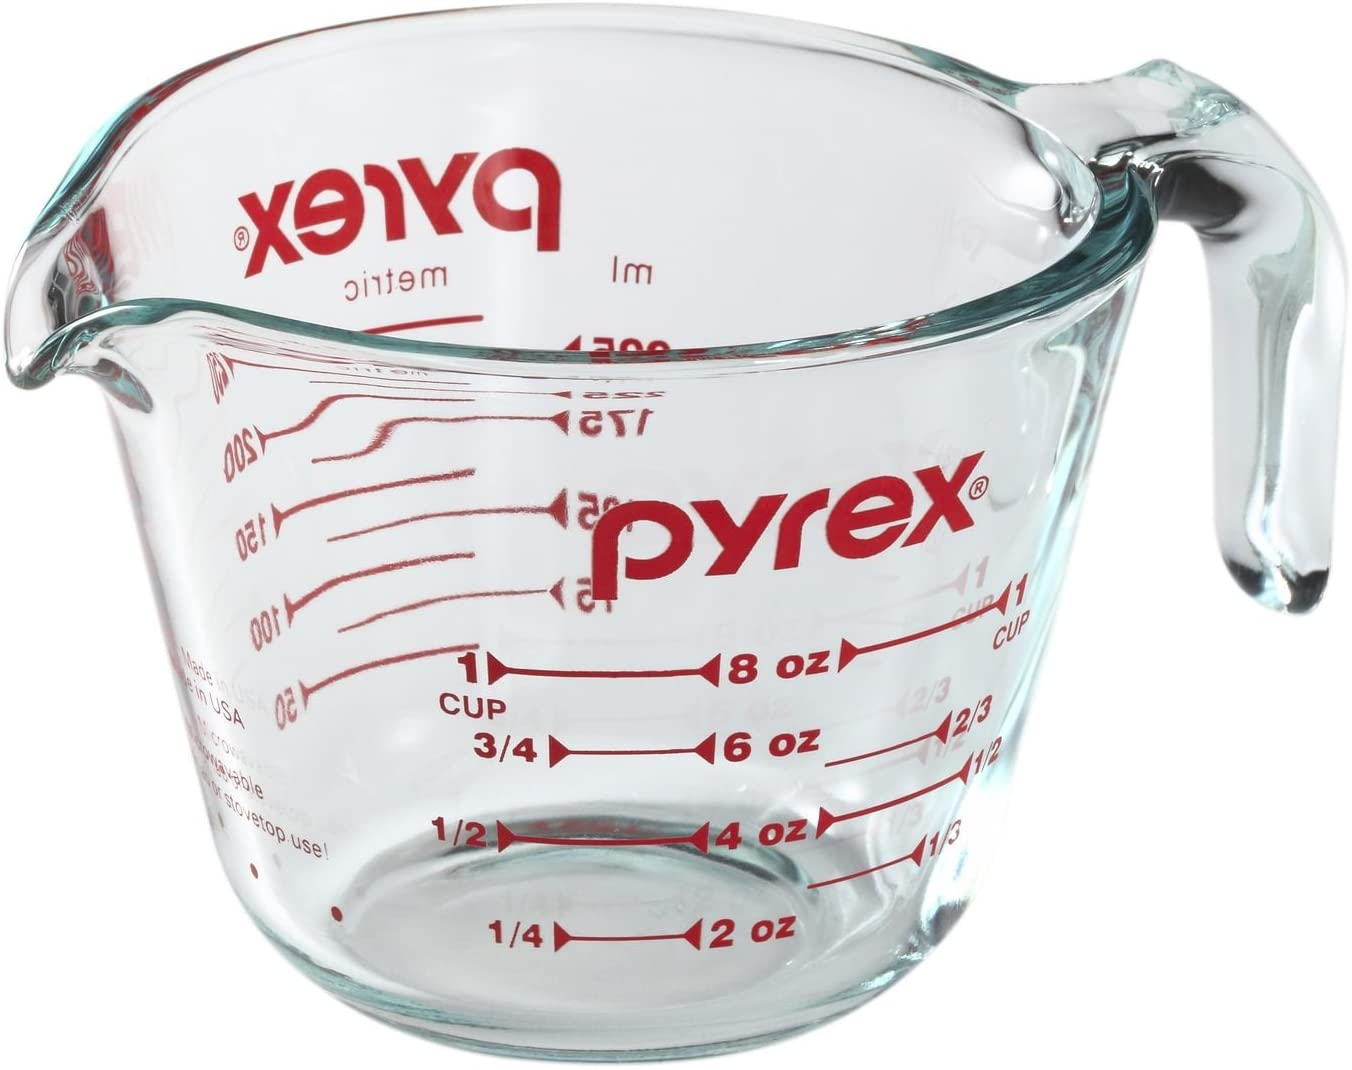
\includegraphics[height=1in]{Silde_Template/images/pyrex.jpg}

\begin{itemize}
    \item A large number of ceramics are stable in both harsh chemical and thermal environments
    \pause
    \item Example Pyrex: resistant to many corrosive chemicals, \pause stable at high temperatures (does not soften until 1,100 K),\pause  and resistant to thermal shock because of its low coefficient of thermal expansion ($33x10^{-7} K^{-1}$)
\end{itemize}
    
\end{frame}

\begin{frame}{Transparent}

\centering
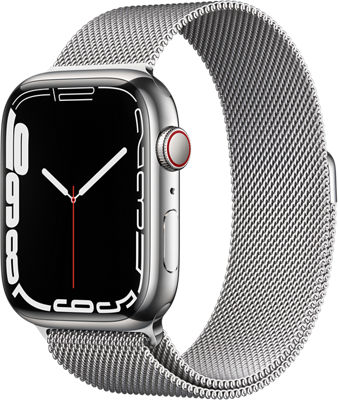
\includegraphics[height=1in]{Silde_Template/images/apple-watch-series-7-lte-45mm-silver-stainless-steel-silver-milanese-loop-mkje3ll-a-sku4790177.jpeg}

\begin{itemize}
    \item Many ceramics are transparent because they have a large $E_g$
    \pause
    \item Examples include sapphire watch covers, precious stones, and optical fibers.
    \pause
    \item Glass optical fibers have percent transmission > 96\%/km
    \pause
    \item "Clearly" not all ceramics are transparent
\end{itemize}
    
\end{frame}

\begin{frame}{Traditional Ceramics}

High volume items such as bricks, tiles, toilet bowls (whitewares), and pottery
\vspace{1em}

\begin{columns}{\textwidth}
  \begin{column}{0.33\textwidth}
    \centering
    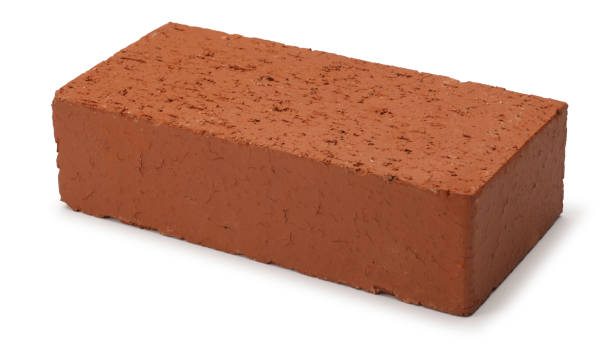
\includegraphics[height=1in]{Silde_Template/images/brick.jpeg}
  \end{column}
  \begin{column}{0.33\textwidth}
  \centering
    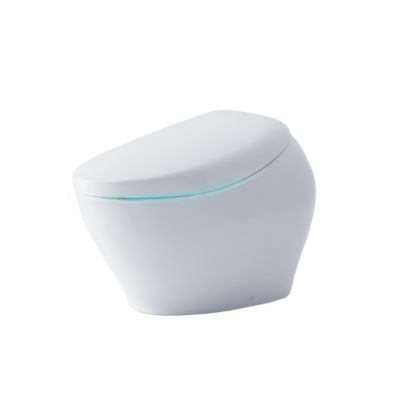
\includegraphics[height=1in]{Silde_Template/images/toilet.jpeg}
  \end{column}
    \begin{column}{0.33\textwidth}
    \centering
    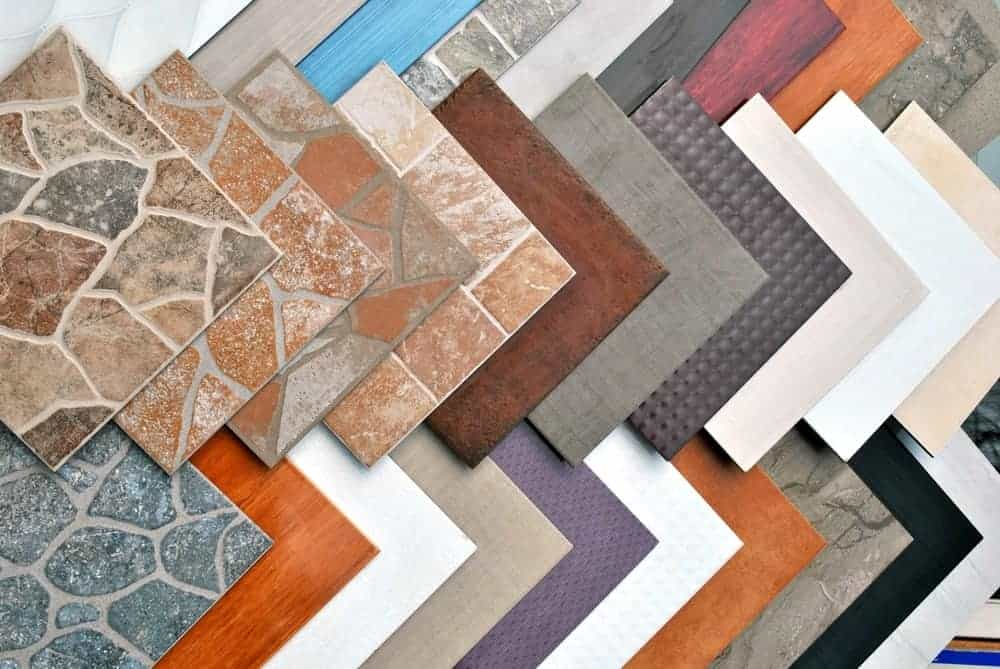
\includegraphics[height=1in]{Silde_Template/images/tiles.jpeg}
  \end{column}
\end{columns}
\pause
\begin{itemize}
    \item Generally based on clay or silica
    \item can require complex processing or tooling
\end{itemize}
\end{frame}

\begin{frame}{Advanced or Technical Ceramics}

\textbf{Advanced Ceramics}
Advanced ceramics are newer materials, such as laser host materials, piezoelectric ceramics, and ceramics
for dynamic random access memories (DRAMs), among others, which are often produced in small quantities at higher prices.    
\vspace{1em}

\begin{columns}
  \begin{column}{0.33\textwidth}
    \centering
    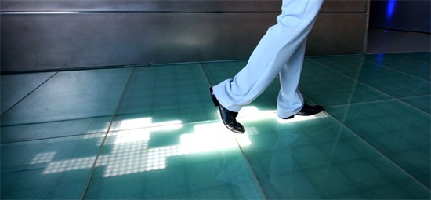
\includegraphics[height=1in]{Silde_Template/images/piezoelectric_floor.png}
  \end{column}
  \begin{column}{0.33\textwidth}
    \centering
    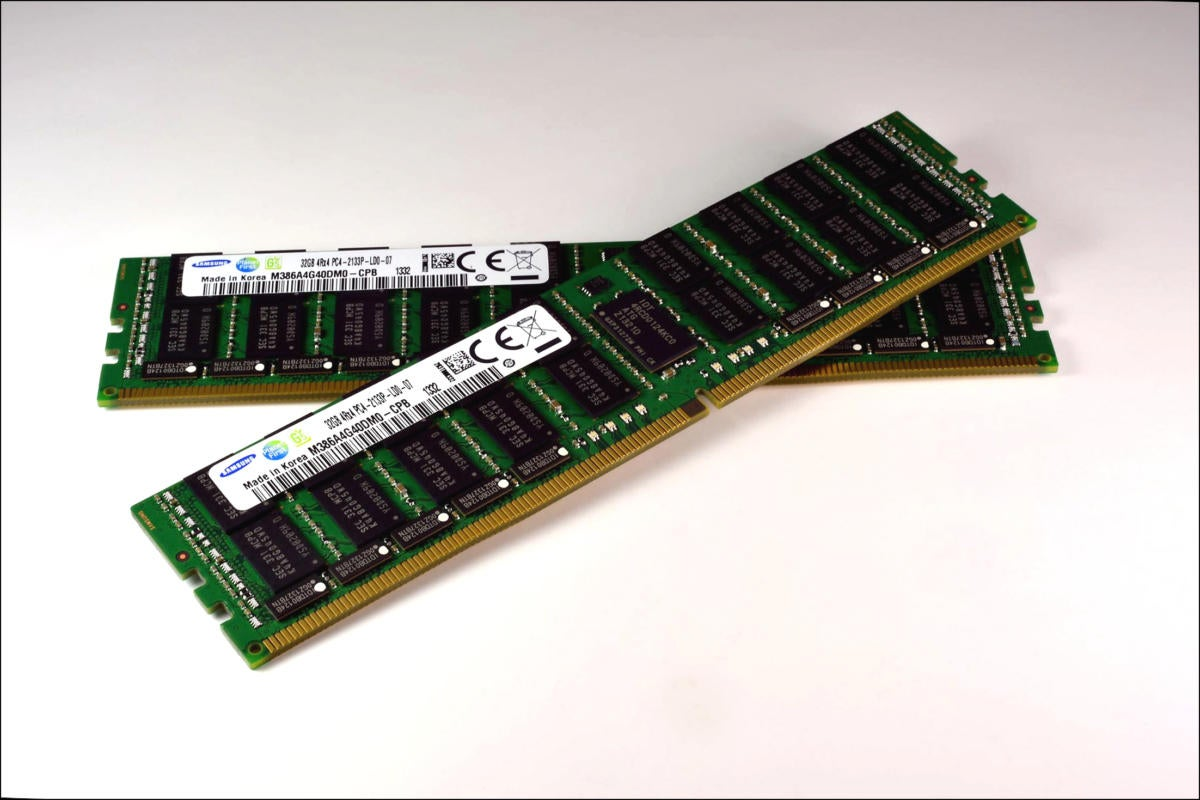
\includegraphics[height=1in]{Silde_Template/images/DRAM.jpeg}
  \end{column}
    \begin{column}{0.33\textwidth}
    \centering
    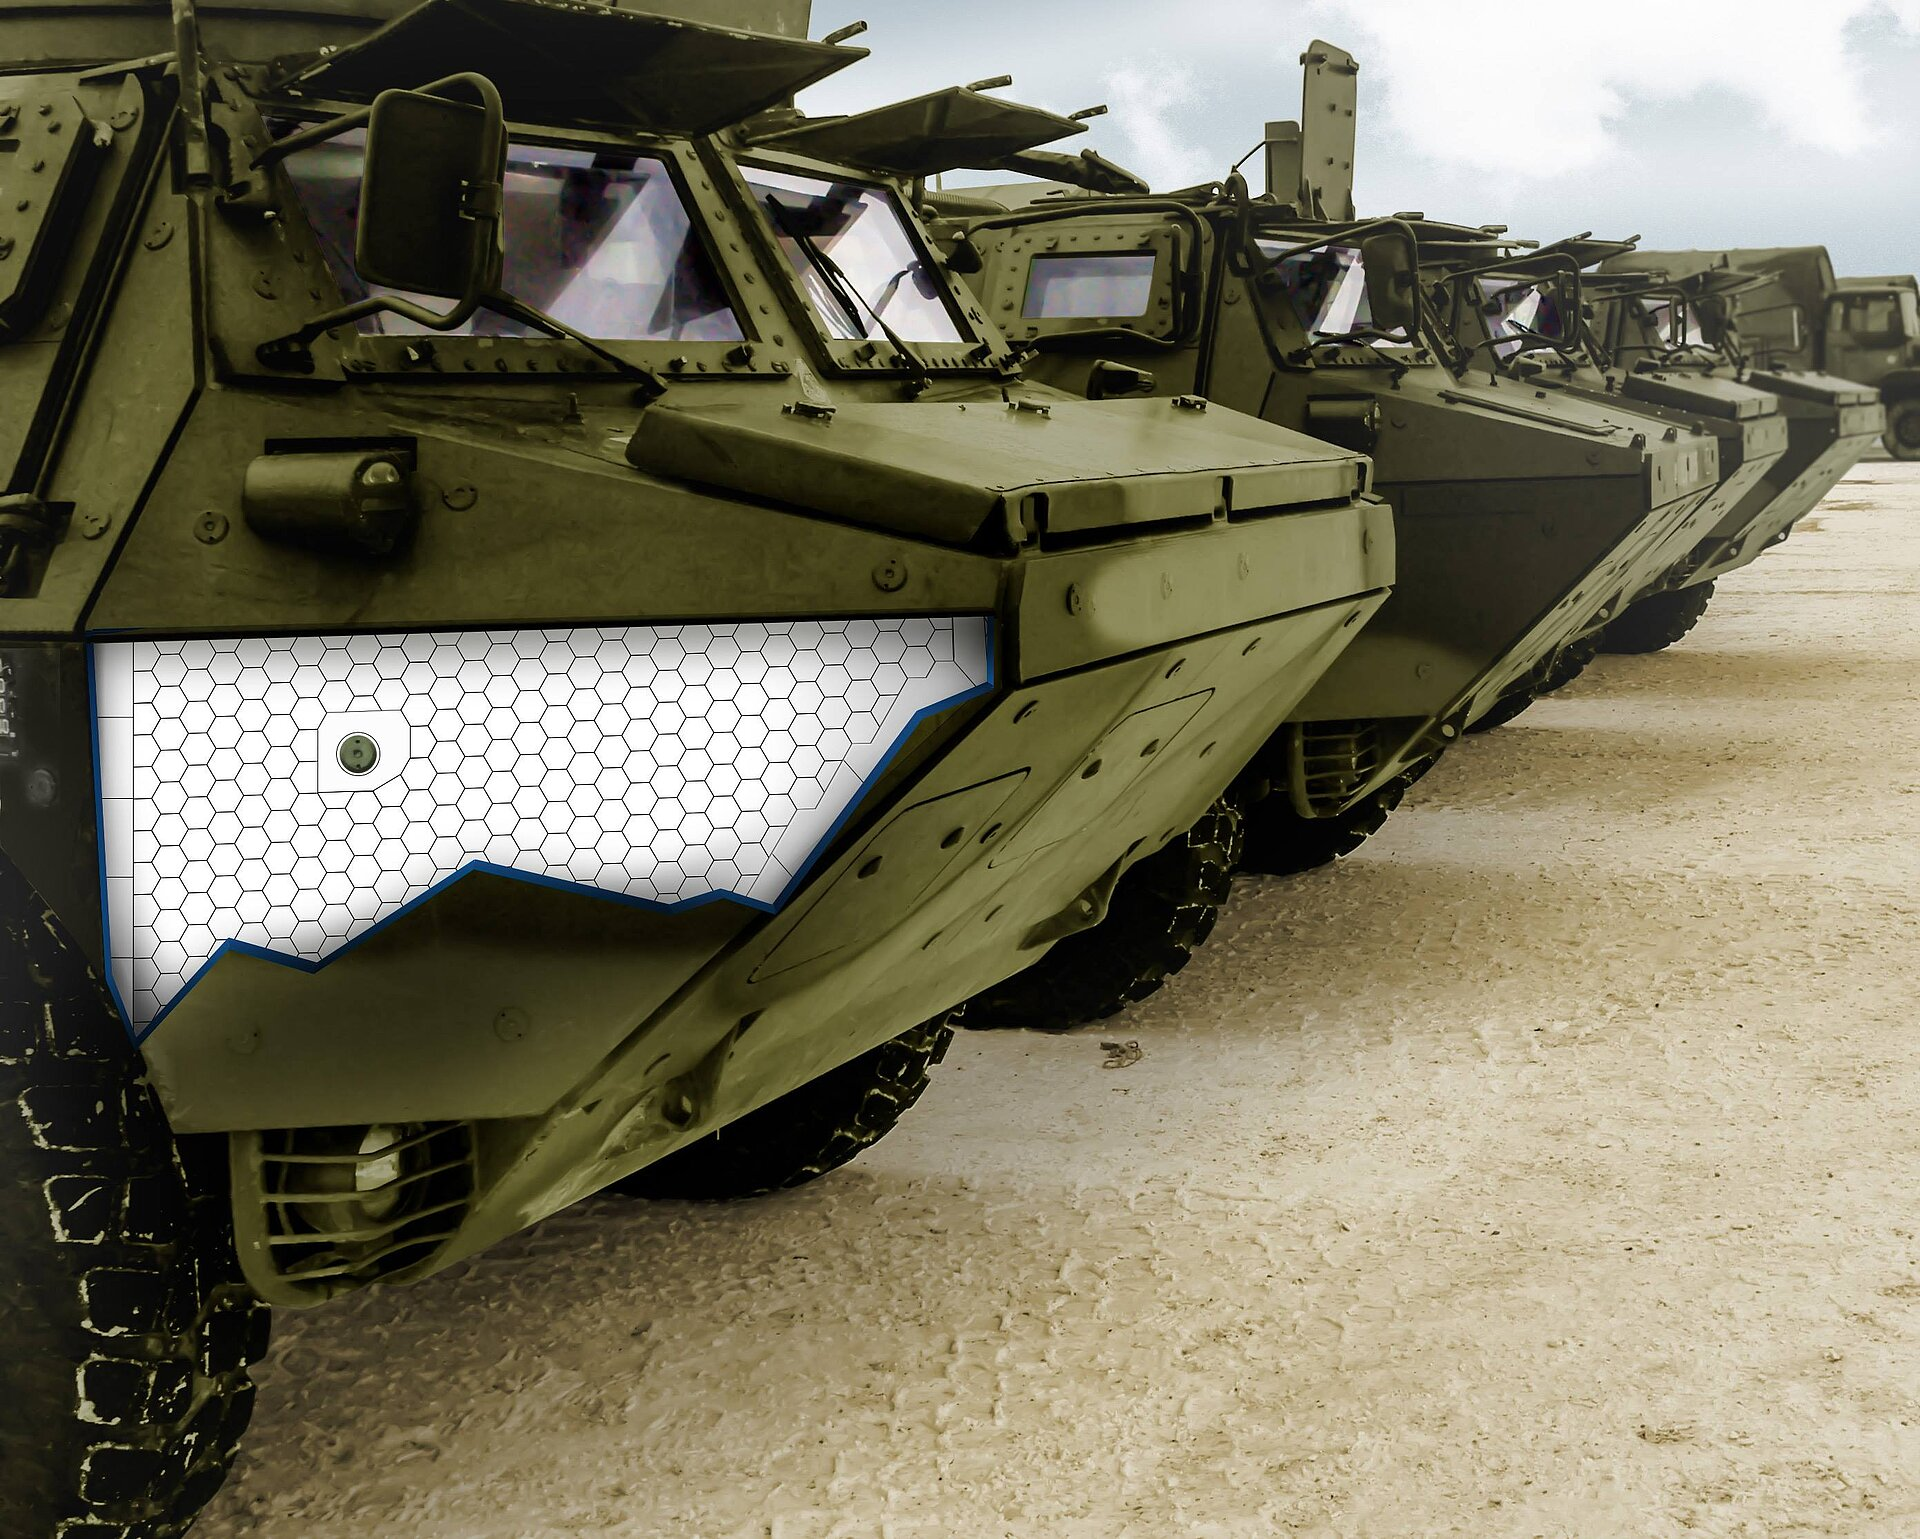
\includegraphics[height=1in]{Silde_Template/images/ballistic ceramics.jpeg}
  \end{column}
\end{columns}
\pause
\vspace{1em}

\begin{itemize}
    \item They exhibit superior mechanical properties, corrosion/oxidation resistance, or electrical, optical and/or magnetic properties.
    \item Emerged primarily over the last 100 years
\end{itemize}

\end{frame}

\begin{frame}{Properties and Applications of Ceramics}
\centering
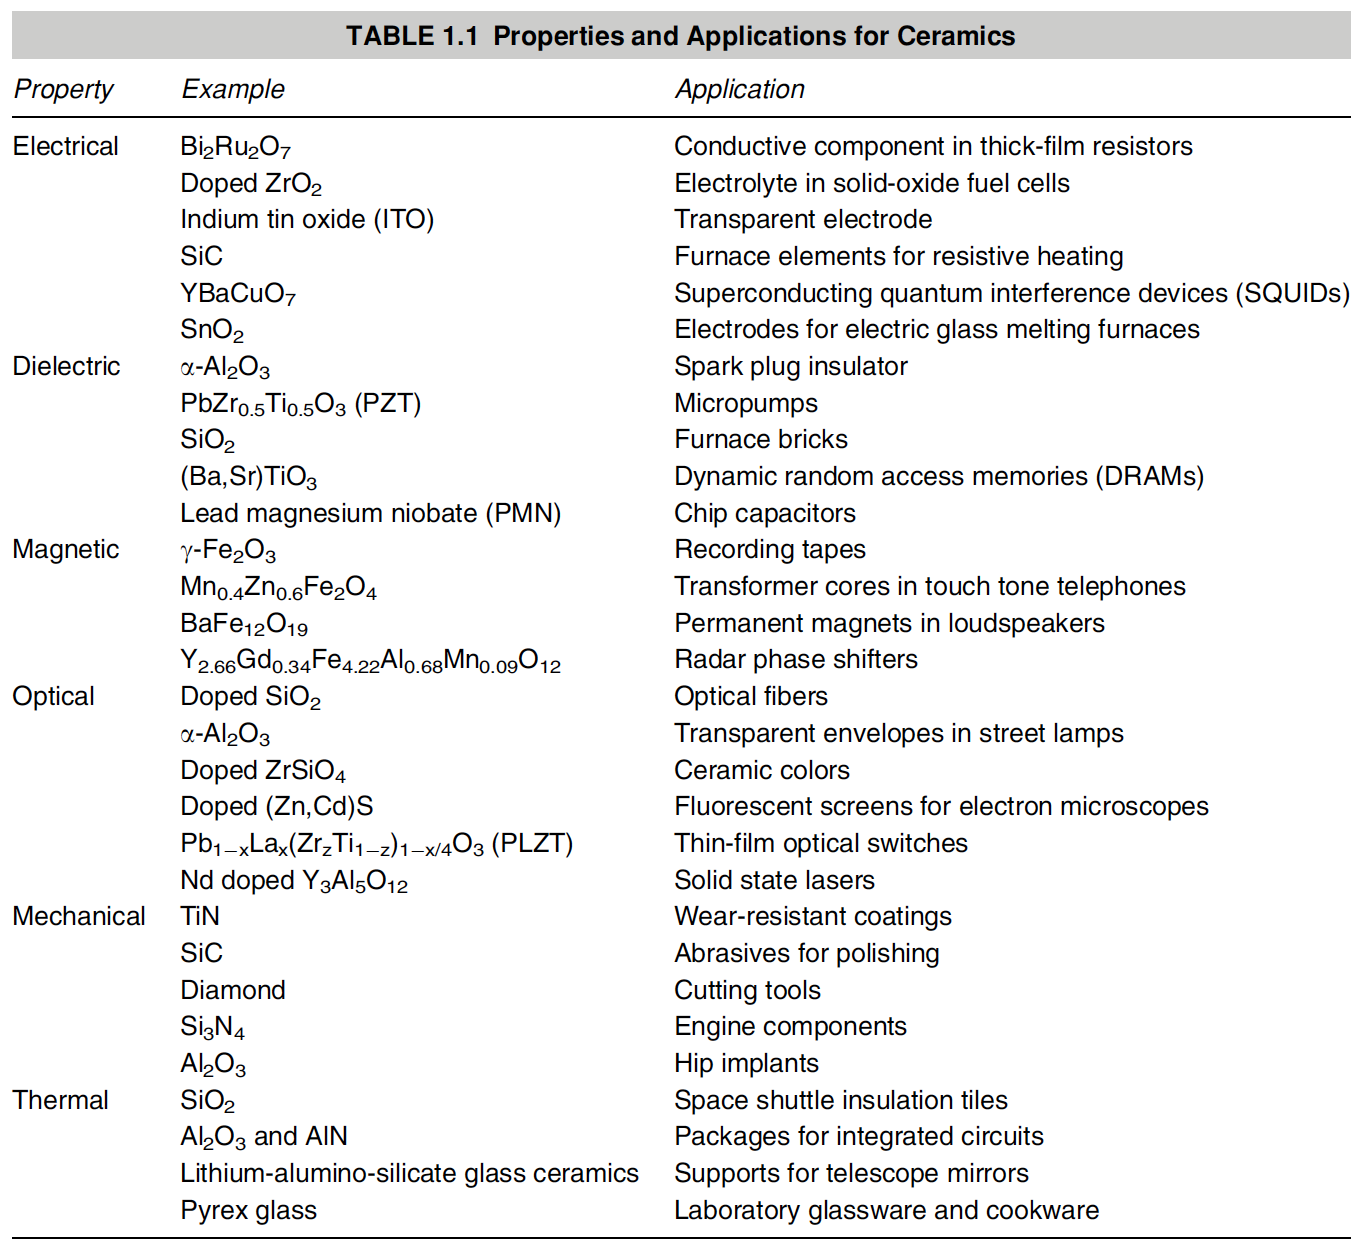
\includegraphics[height=\textheight]{Silde_Template/images/Properties of ceramics.png}
\end{frame}

\begin{frame}{Advanced vs. Traditional Ceramics}
\centering
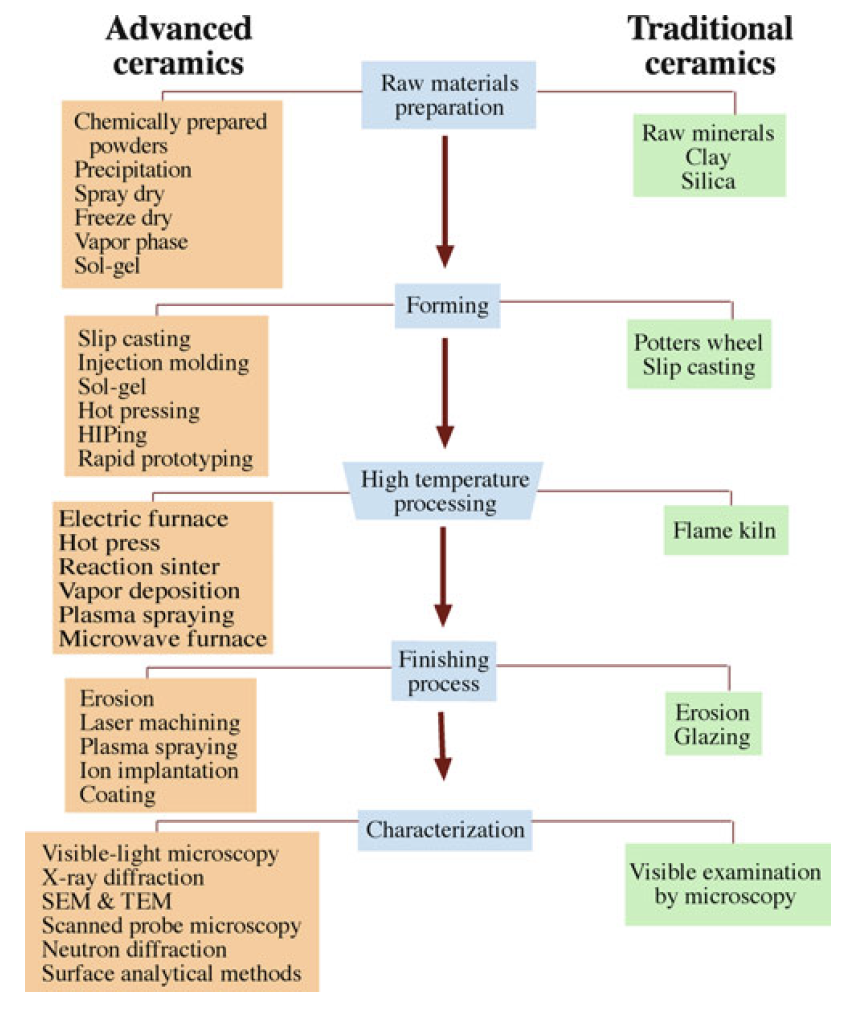
\includegraphics[height=0.8\textheight]{Silde_Template/images/Comparison.png}
\end{frame}

\section{Market and Future}

\begin{frame}{Overall Market Finances}
Ceramics is a multibillion-dollar industry. Worldwide sales are about \$100 billion per year; the U.S. market alone is over \$35 billion annually.
\vspace{1em}

\centering
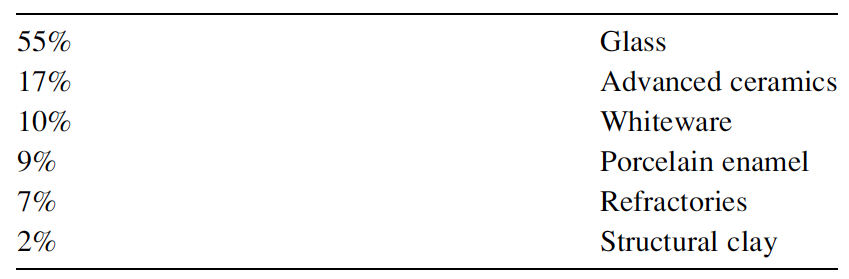
\includegraphics[width=0.75\textwidth]{Silde_Template/images/general market.png}
\vspace{1em}

\begin{itemize}
    \item Bricks and glass, the commodity ceramics have the largest market
\end{itemize}
    
\end{frame}

\begin{frame}{Advanced Ceramics}
\vspace{1em}

\centering
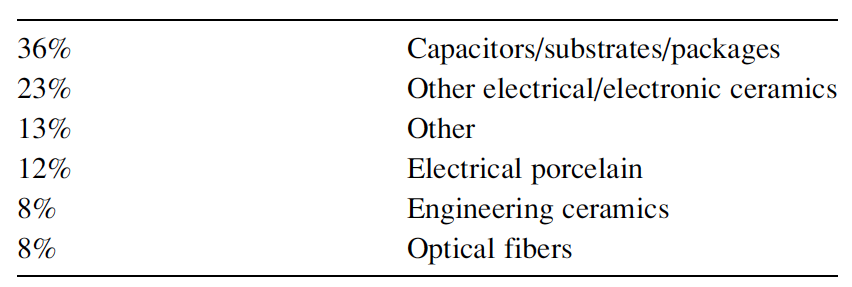
\includegraphics[width=0.6\textwidth]{Silde_Template/images/advanced ceramics.png}

\begin{itemize}
    \small
    \item More than half of this sector is comprised of electrical and electronic ceramics and ceramic packages \pause
    \item Significant growth areas include microwave filters and resonators for use in wireless communication \pause
    \item Engineering ceramics, also called structural ceramics, include wear-resistant components such as dies, nozzles,and bearings\pause
    \item Bioceramics (e.g., ceramic and glass-ceramic implants and dental crowns) account for about 20\% of this market (dental crowns) \pause 
    \item Porcelain enamel is the ceramic coating applied to many steel appliances such as kitchen stoves, washers and dryers \pause
    \item More than 50\% of refractories are consumed by the steel industry \pause
\end{itemize}
\end{frame}

\begin{frame}{Structural Ceramics}
    \centering
    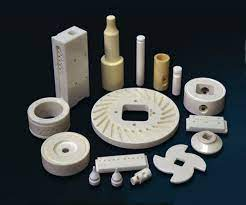
\includegraphics[height=1in]{Silde_Template/images/Structural_Ceramics.jpg}
\begin{itemize}
    \item Include silicon nitride ($Si_3N_4$), silicon carbide ($SiC$), zirconia ($ZrO_2$), boron carbide ($B_4C$), and alumina ($Al_2O_3$)
    \pause
    \item They are used in applications such as cutting tools, wear components, heat exchangers, and engine parts
    \pause
    \item The relevant properties of structural ceramics are high hardness, low density, high-temperature mechanical strength, creep resistance, corrosion resistance, and chemical inertness
    \pause
\end{itemize}
\vspace{1em}

\textbf{Key Issues}
\begin{itemize}
    \item Reducing the cost of the final product
    \item Improving reliability
    \item Improving reproducibility
\end{itemize}

\end{frame}

\begin{frame}{Electrical Ceramics}

\centering
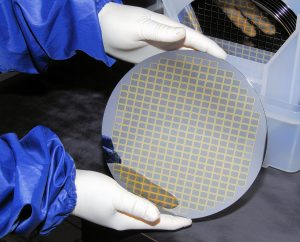
\includegraphics[height=1in]{Silde_Template/images/Wafer.jpg}

\begin{itemize}
    \item Include barium titanate ($BaTiO_3$), zinc oxide ($ZnO$), lead zirconate titanate [$Pb(Zr_xTi_{1-x})O_3$], aluminum nitride ($AlN$), and high-temperature superconductors \pause
    \item They are used in applications as diverse as capacitor dielectrics, varistors, micro-electro-mechanical systems (MEMS), substrates, and packages for integrated circuits \pause
\end{itemize}

\textbf{Key Issues}
\begin{itemize}
    \item Integrating with existing semiconductor technology
    \item Improving processing
    \item Enhancing compatibility with other materials
    \item Improved electrical resistivity in thin films
\end{itemize}

\end{frame}

\begin{frame}{Bioceramics}
    \centering
    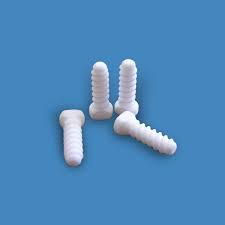
\includegraphics[height=1in]{Silde_Template/images/bioceramic Screw.jpg}

\begin{itemize}
    \item The response of these materials varies from nearly inert to bioactive to resorbable \pause
    \item Nearly inert bioceramics include alumina ($Al_2O_3$) and zirconia ($ZrO_2$) \pause
    \item Bioactive ceramics include hydroxyapatite and some special glass and glass-ceramic formulations \pause
    \item Tricalcium phosphate, which dissolves in the body, is an example of a resorbable bioceramic \pause
\end{itemize}

\textbf{Key Issues}
\begin{itemize}
    \item Matching mechanical properties to human tissues
    \item Enhancing compatibility with other materials
    \item Improving processing methods and reliability 
\end{itemize}
    
\end{frame}

\begin{frame}{Coating and Films}
    \centering
    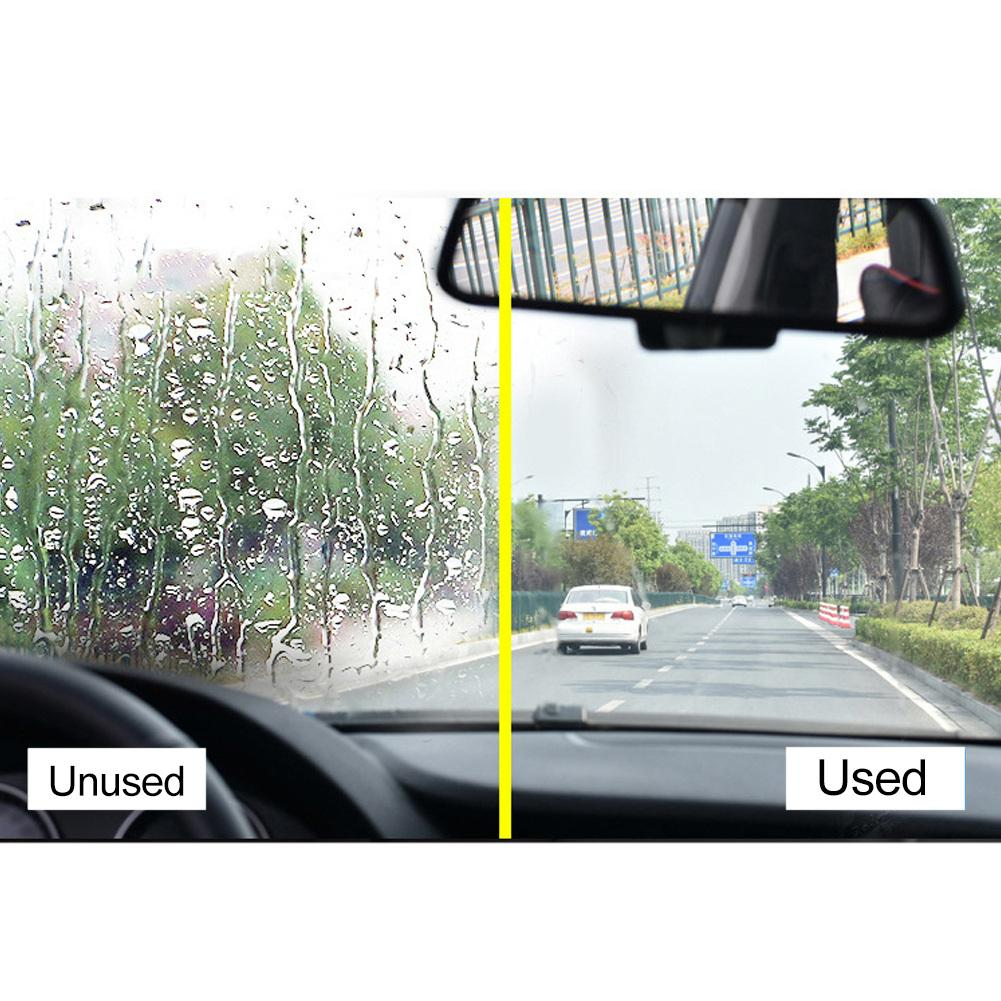
\includegraphics[height=1in]{Silde_Template/images/ceramic_coating_glass.jpg}
    \begin{itemize}
        \item Coatings and films modify the surface properties of a material (e.g., a bioactive coating deposited on a bio-inert implant) \pause
        \item Economic reasons: Apply a coating of an expensive material on a lower cost substrate rather than make the component entirely from the more expensive material \pause $\rightarrow$ An example is applying a diamond coating on a cutting tool \pause
        \item Thin film properties can be better, the transport properties of thin films of HTSCs, which are improved over the bulk
    \end{itemize}


\textbf{Key Issues}
\begin{itemize}
    \item Understanding film deposition and growth
    \item Improving film/substrate adhesion
    \item Increasing reproducibility
\end{itemize}

\end{frame}

\begin{frame}{Composites}
    \centering
    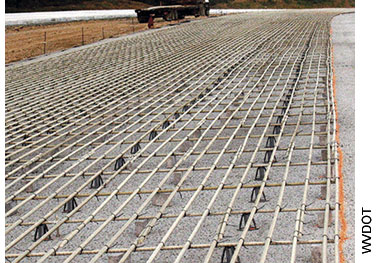
\includegraphics[height=.7in]{Silde_Template/images/rebarb.jpg}
\begin{itemize}
    \item Composites may use ceramics as the matrix phase and/or the reinforcing phase \pause
    \item Composite display a combination of the preferred characteristics of each of the components \pause
    \item Ceramic matrix composites increase fracture toughness through reinforcement with whiskers or fibers \pause
    \item Metal matrix composites increase in strength, enhanced creep resistance, and greater wear resistance \pause
\end{itemize}

\textbf{Key Issues}
\begin{itemize}
    \item Reducing processing costs
    \item Developing compatible combinations of materials (e.g., matching coefficients of thermal expansion)
    \item Understanding interfaces
\end{itemize}

\end{frame}

\begin{frame}{Nanoceramics}
\centering
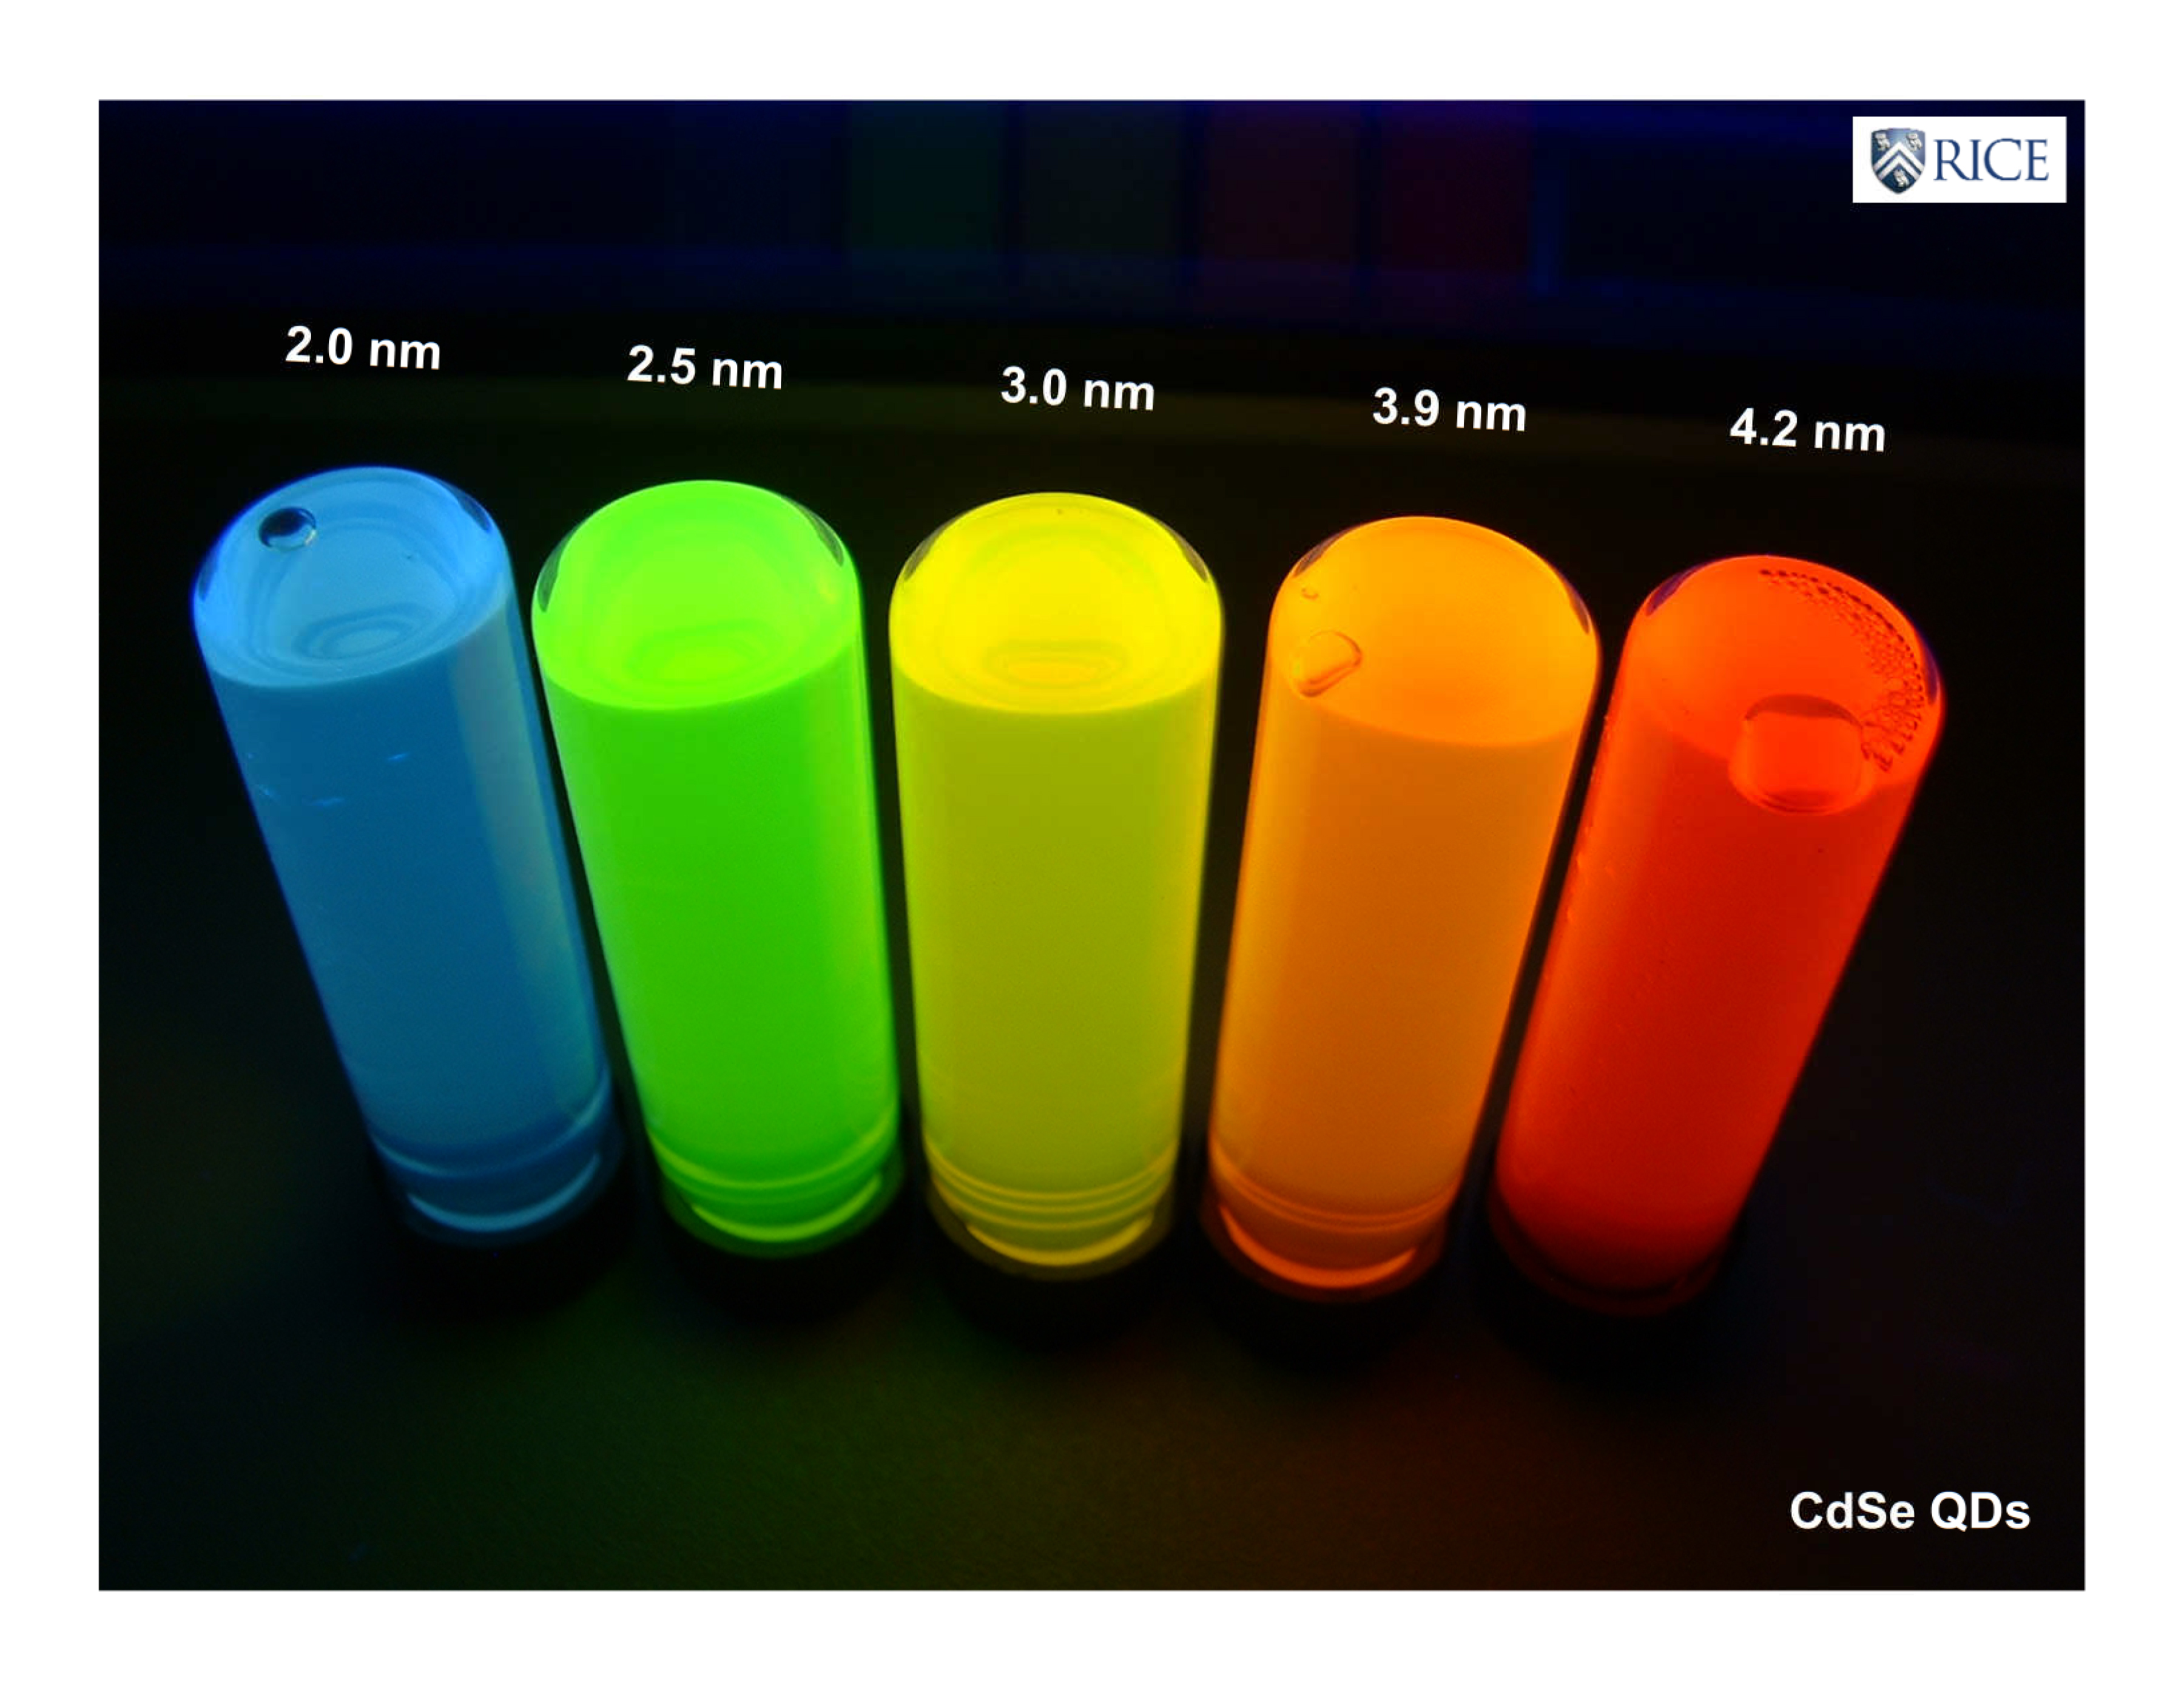
\includegraphics[height=1in]{Silde_Template/images/CdSe_Quantum_Dots.jpg}
\begin{itemize}
    \item Widely used in cosmetic products (e.g., sunscreens), as stabilizers, and they are critical in many catalytic applications \pause
    \item Modern applications in quantum dots, fuel cells, and specialty coating applications \pause
\end{itemize}

\textbf{Key Issues}
\begin{itemize}
    \item Making them
    \item Integrating them into devices through either top-down or bottom-up approaches
    \item Ensuring that they do not have a negative impact on society
\end{itemize}

\end{frame}

\section{Important concepts to master}
\begin{frame}{Important Concepts to Master}
\begin{itemize}
    \item How to determine if a materials is a ceramic or not? \pause
    \item An explanation of the range and diversity of properties that ceramics can exhibit. For example, ceramics have some of the lowest and highest thermal conductivity.  \pause
    \item A working knowledge of what applications ceramic materials are used for. What about their properties makes them useful for these applications? 
\end{itemize}
\end{frame}
\end{document}



        
